% Sinh tự động bởi report/scripts/ve_hinh_bitboard.py, đừng sửa tay.
\definecolor{bbX}{HTML}{1F4E8C}
\definecolor{bbO}{HTML}{C8553D}
\definecolor{bbKq}{HTML}{2E8B57}
\definecolor{bbSai}{HTML}{D7263D}
\definecolor{bbMat}{HTML}{DCE8F5}
\definecolor{bbVang}{HTML}{FBE7A1}
\definecolor{bbXam}{HTML}{BDBDBD}
\definecolor{bbNhat}{HTML}{9CC3E6}
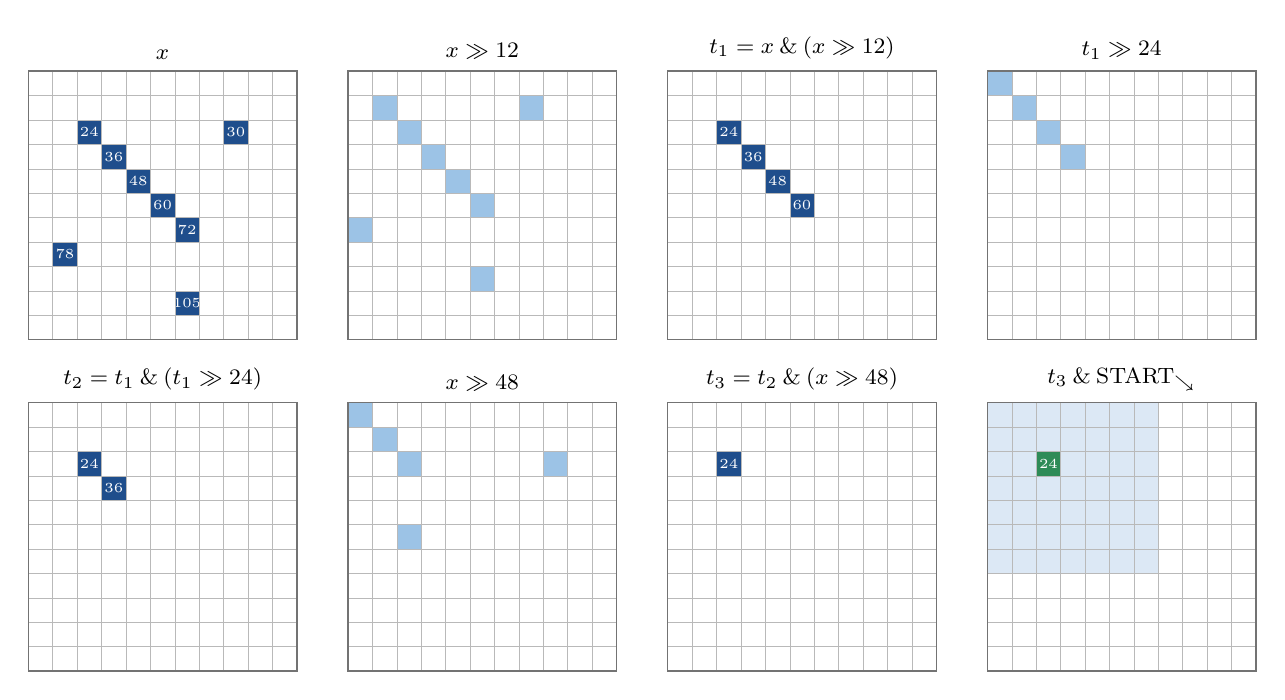
\begin{tikzpicture}
\begin{scope}[shift={(0.000,0.000)}]
\fill[bbX] (0.620,-0.620) rectangle ++(0.310,-0.310);
\node[text=white,inner sep=0,font=\fontsize{5}{5}\selectfont] at (0.775,-0.775) {24};
\fill[bbX] (2.480,-0.620) rectangle ++(0.310,-0.310);
\node[text=white,inner sep=0,font=\fontsize{5}{5}\selectfont] at (2.635,-0.775) {30};
\fill[bbX] (0.930,-0.930) rectangle ++(0.310,-0.310);
\node[text=white,inner sep=0,font=\fontsize{5}{5}\selectfont] at (1.085,-1.085) {36};
\fill[bbX] (1.240,-1.240) rectangle ++(0.310,-0.310);
\node[text=white,inner sep=0,font=\fontsize{5}{5}\selectfont] at (1.395,-1.395) {48};
\fill[bbX] (1.550,-1.550) rectangle ++(0.310,-0.310);
\node[text=white,inner sep=0,font=\fontsize{5}{5}\selectfont] at (1.705,-1.705) {60};
\fill[bbX] (1.860,-1.860) rectangle ++(0.310,-0.310);
\node[text=white,inner sep=0,font=\fontsize{5}{5}\selectfont] at (2.015,-2.015) {72};
\fill[bbX] (0.310,-2.170) rectangle ++(0.310,-0.310);
\node[text=white,inner sep=0,font=\fontsize{5}{5}\selectfont] at (0.465,-2.325) {78};
\fill[bbX] (1.860,-2.790) rectangle ++(0.310,-0.310);
\node[text=white,inner sep=0,font=\fontsize{5}{5}\selectfont] at (2.015,-2.945) {105};
\draw[gray!55,line width=.2pt] (0,0) grid[step=0.310] (3.410,-3.410);
\draw[gray!90!black,line width=.5pt] (0,0) rectangle (3.410,-3.410);
\node[anchor=south,font=\footnotesize] at (1.705,0.03) {$x$};
\end{scope}
\begin{scope}[shift={(4.060,0.000)}]
\fill[bbNhat] (0.310,-0.310) rectangle ++(0.310,-0.310);
\fill[bbNhat] (2.170,-0.310) rectangle ++(0.310,-0.310);
\fill[bbNhat] (0.620,-0.620) rectangle ++(0.310,-0.310);
\fill[bbNhat] (0.930,-0.930) rectangle ++(0.310,-0.310);
\fill[bbNhat] (1.240,-1.240) rectangle ++(0.310,-0.310);
\fill[bbNhat] (1.550,-1.550) rectangle ++(0.310,-0.310);
\fill[bbNhat] (0.000,-1.860) rectangle ++(0.310,-0.310);
\fill[bbNhat] (1.550,-2.480) rectangle ++(0.310,-0.310);
\draw[gray!55,line width=.2pt] (0,0) grid[step=0.310] (3.410,-3.410);
\draw[gray!90!black,line width=.5pt] (0,0) rectangle (3.410,-3.410);
\node[anchor=south,font=\footnotesize] at (1.705,0.03) {$x \gg 12$};
\end{scope}
\begin{scope}[shift={(8.120,0.000)}]
\fill[bbX] (0.620,-0.620) rectangle ++(0.310,-0.310);
\node[text=white,inner sep=0,font=\fontsize{5}{5}\selectfont] at (0.775,-0.775) {24};
\fill[bbX] (0.930,-0.930) rectangle ++(0.310,-0.310);
\node[text=white,inner sep=0,font=\fontsize{5}{5}\selectfont] at (1.085,-1.085) {36};
\fill[bbX] (1.240,-1.240) rectangle ++(0.310,-0.310);
\node[text=white,inner sep=0,font=\fontsize{5}{5}\selectfont] at (1.395,-1.395) {48};
\fill[bbX] (1.550,-1.550) rectangle ++(0.310,-0.310);
\node[text=white,inner sep=0,font=\fontsize{5}{5}\selectfont] at (1.705,-1.705) {60};
\draw[gray!55,line width=.2pt] (0,0) grid[step=0.310] (3.410,-3.410);
\draw[gray!90!black,line width=.5pt] (0,0) rectangle (3.410,-3.410);
\node[anchor=south,font=\footnotesize] at (1.705,0.03) {$t_1 = x \mathbin{\&} (x \gg 12)$};
\end{scope}
\begin{scope}[shift={(12.180,0.000)}]
\fill[bbNhat] (0.000,0.000) rectangle ++(0.310,-0.310);
\fill[bbNhat] (0.310,-0.310) rectangle ++(0.310,-0.310);
\fill[bbNhat] (0.620,-0.620) rectangle ++(0.310,-0.310);
\fill[bbNhat] (0.930,-0.930) rectangle ++(0.310,-0.310);
\draw[gray!55,line width=.2pt] (0,0) grid[step=0.310] (3.410,-3.410);
\draw[gray!90!black,line width=.5pt] (0,0) rectangle (3.410,-3.410);
\node[anchor=south,font=\footnotesize] at (1.705,0.03) {$t_1 \gg 24$};
\end{scope}
\begin{scope}[shift={(0.000,-4.210)}]
\fill[bbX] (0.620,-0.620) rectangle ++(0.310,-0.310);
\node[text=white,inner sep=0,font=\fontsize{5}{5}\selectfont] at (0.775,-0.775) {24};
\fill[bbX] (0.930,-0.930) rectangle ++(0.310,-0.310);
\node[text=white,inner sep=0,font=\fontsize{5}{5}\selectfont] at (1.085,-1.085) {36};
\draw[gray!55,line width=.2pt] (0,0) grid[step=0.310] (3.410,-3.410);
\draw[gray!90!black,line width=.5pt] (0,0) rectangle (3.410,-3.410);
\node[anchor=south,font=\footnotesize] at (1.705,0.03) {$t_2 = t_1 \mathbin{\&} (t_1 \gg 24)$};
\end{scope}
\begin{scope}[shift={(4.060,-4.210)}]
\fill[bbNhat] (0.000,0.000) rectangle ++(0.310,-0.310);
\fill[bbNhat] (0.310,-0.310) rectangle ++(0.310,-0.310);
\fill[bbNhat] (0.620,-0.620) rectangle ++(0.310,-0.310);
\fill[bbNhat] (2.480,-0.620) rectangle ++(0.310,-0.310);
\fill[bbNhat] (0.620,-1.550) rectangle ++(0.310,-0.310);
\draw[gray!55,line width=.2pt] (0,0) grid[step=0.310] (3.410,-3.410);
\draw[gray!90!black,line width=.5pt] (0,0) rectangle (3.410,-3.410);
\node[anchor=south,font=\footnotesize] at (1.705,0.03) {$x \gg 48$};
\end{scope}
\begin{scope}[shift={(8.120,-4.210)}]
\fill[bbX] (0.620,-0.620) rectangle ++(0.310,-0.310);
\node[text=white,inner sep=0,font=\fontsize{5}{5}\selectfont] at (0.775,-0.775) {24};
\draw[gray!55,line width=.2pt] (0,0) grid[step=0.310] (3.410,-3.410);
\draw[gray!90!black,line width=.5pt] (0,0) rectangle (3.410,-3.410);
\node[anchor=south,font=\footnotesize] at (1.705,0.03) {$t_3 = t_2 \mathbin{\&} (x \gg 48)$};
\end{scope}
\begin{scope}[shift={(12.180,-4.210)}]
\fill[bbMat] (0.000,0.000) rectangle ++(0.310,-0.310);
\fill[bbMat] (0.310,0.000) rectangle ++(0.310,-0.310);
\fill[bbMat] (0.620,0.000) rectangle ++(0.310,-0.310);
\fill[bbMat] (0.930,0.000) rectangle ++(0.310,-0.310);
\fill[bbMat] (1.240,0.000) rectangle ++(0.310,-0.310);
\fill[bbMat] (1.550,0.000) rectangle ++(0.310,-0.310);
\fill[bbMat] (1.860,0.000) rectangle ++(0.310,-0.310);
\fill[bbMat] (0.000,-0.310) rectangle ++(0.310,-0.310);
\fill[bbMat] (0.310,-0.310) rectangle ++(0.310,-0.310);
\fill[bbMat] (0.620,-0.310) rectangle ++(0.310,-0.310);
\fill[bbMat] (0.930,-0.310) rectangle ++(0.310,-0.310);
\fill[bbMat] (1.240,-0.310) rectangle ++(0.310,-0.310);
\fill[bbMat] (1.550,-0.310) rectangle ++(0.310,-0.310);
\fill[bbMat] (1.860,-0.310) rectangle ++(0.310,-0.310);
\fill[bbMat] (0.000,-0.620) rectangle ++(0.310,-0.310);
\fill[bbMat] (0.310,-0.620) rectangle ++(0.310,-0.310);
\fill[bbKq] (0.620,-0.620) rectangle ++(0.310,-0.310);
\node[text=white,inner sep=0,font=\fontsize{5}{5}\selectfont] at (0.775,-0.775) {24};
\fill[bbMat] (0.930,-0.620) rectangle ++(0.310,-0.310);
\fill[bbMat] (1.240,-0.620) rectangle ++(0.310,-0.310);
\fill[bbMat] (1.550,-0.620) rectangle ++(0.310,-0.310);
\fill[bbMat] (1.860,-0.620) rectangle ++(0.310,-0.310);
\fill[bbMat] (0.000,-0.930) rectangle ++(0.310,-0.310);
\fill[bbMat] (0.310,-0.930) rectangle ++(0.310,-0.310);
\fill[bbMat] (0.620,-0.930) rectangle ++(0.310,-0.310);
\fill[bbMat] (0.930,-0.930) rectangle ++(0.310,-0.310);
\fill[bbMat] (1.240,-0.930) rectangle ++(0.310,-0.310);
\fill[bbMat] (1.550,-0.930) rectangle ++(0.310,-0.310);
\fill[bbMat] (1.860,-0.930) rectangle ++(0.310,-0.310);
\fill[bbMat] (0.000,-1.240) rectangle ++(0.310,-0.310);
\fill[bbMat] (0.310,-1.240) rectangle ++(0.310,-0.310);
\fill[bbMat] (0.620,-1.240) rectangle ++(0.310,-0.310);
\fill[bbMat] (0.930,-1.240) rectangle ++(0.310,-0.310);
\fill[bbMat] (1.240,-1.240) rectangle ++(0.310,-0.310);
\fill[bbMat] (1.550,-1.240) rectangle ++(0.310,-0.310);
\fill[bbMat] (1.860,-1.240) rectangle ++(0.310,-0.310);
\fill[bbMat] (0.000,-1.550) rectangle ++(0.310,-0.310);
\fill[bbMat] (0.310,-1.550) rectangle ++(0.310,-0.310);
\fill[bbMat] (0.620,-1.550) rectangle ++(0.310,-0.310);
\fill[bbMat] (0.930,-1.550) rectangle ++(0.310,-0.310);
\fill[bbMat] (1.240,-1.550) rectangle ++(0.310,-0.310);
\fill[bbMat] (1.550,-1.550) rectangle ++(0.310,-0.310);
\fill[bbMat] (1.860,-1.550) rectangle ++(0.310,-0.310);
\fill[bbMat] (0.000,-1.860) rectangle ++(0.310,-0.310);
\fill[bbMat] (0.310,-1.860) rectangle ++(0.310,-0.310);
\fill[bbMat] (0.620,-1.860) rectangle ++(0.310,-0.310);
\fill[bbMat] (0.930,-1.860) rectangle ++(0.310,-0.310);
\fill[bbMat] (1.240,-1.860) rectangle ++(0.310,-0.310);
\fill[bbMat] (1.550,-1.860) rectangle ++(0.310,-0.310);
\fill[bbMat] (1.860,-1.860) rectangle ++(0.310,-0.310);
\draw[gray!55,line width=.2pt] (0,0) grid[step=0.310] (3.410,-3.410);
\draw[gray!90!black,line width=.5pt] (0,0) rectangle (3.410,-3.410);
\node[anchor=south,font=\footnotesize] at (1.705,0.03) {$t_3 \mathbin{\&} \mathrm{START}_{\searrow}$};
\end{scope}
\end{tikzpicture}
